\chapter{Introduction}
\graphicspath{{Chapter1/Figs/}{Chapter1/Figs/}}

This chapter introduces the reader to this thesis's primary focus, key topics, and broad explanations. It also displays the supposition, goals, and objectives of the thesis's primary content and structure.

\section{Background}
\label{chapter1-background}

There has been a long-standing interest in developing neural interfaces, systems that sense and interact with the nervous system's electrical activity. Successful research into the development of technologies that enable neural interfacing has been going on for decades, with the first experiments being conducted by Jacques J. Vidal in the late 1970s \citep{vidal_real-time_1977}. In particular, a related discipline focusing on the direct interaction between brains and computers via a brain-computer interface (BCI) has accumulated much momentum with the emergence of popular companies such as Neuralink \citep{mor_brain-computer_2021}.

One aspect of BCIs is the development of imaging technologies that enable the measurement of brain activity. A distinction can be made between different methods of measuring brain activity signals at different locations, i.e. invasive sensors, such as in electrocorticography (ECoG), a sensor-based\footnote{Other options next to sensor-based imaging methods are e.g. scan-based methods such as computed tomography (CAT) that utilises special x-rays to produce axial images of the brain.} imaging method which uses electrodes placed on the surface of the brain, or non-invasively placed sensors on the body, such as in electroencephalography (EEG). Both methods measure the electrical field elicited by the firing of neuronal populations; however, with decreasing spatial precision, the farther the electrode is placed from the brain and the more tissues (e.g., bones) are between firing neurons and the measuring sensor.

The other aspect is the development of software that reads and interprets data from sensors. Both aspects present their own set of challenges and complexities. Nonetheless, complete and applicable BCIs work in practice and have been used for many years in patients with neurological disorders \citep{braingate_publications_nodate}. There are also consumer and non-clinical BCIs available, such as the OpenBCI and Neurosity products, which aim to democratise the use of EEG systems by offering low-cost hardware and open-source software.

\section{Relevance}
\label{chapter1-relevance}

The possibilities for sufficiently and directly connecting the human brain to the outside world via or with computers are seemingly endless, given the (purely physical\footnote{There is research on the quantum mind that describes how classical mechanics cannot explain consciousness; however, this is not taken into account in this thesis because this research is still in its early stages.}) assertion that all of our feelings, memories, dreams, and thoughts are most likely the sum of electrical activities in our brain. There are several use cases for utilising insights from our brain to interface with computers, such as controlling prosthetic limbs for amputees \citep{campbell_amputee_2014} as shown on \autoref{fig:prostetic-arms}, enabling communication for people with locked-in syndrome\footnote{Locked-in syndrome describes the paralysis of all voluntary muscles in its entirety, therefore making it impossible for people to communicate with the outside world.} \citep{chaudhary_spelling_2022}, or diagnosing neurological problems and improving the mental capacities of elderly patients \citep{belkacem_brain_2020} are promising examples, to name a few.

\begin{figure}[ht]
  \centering
  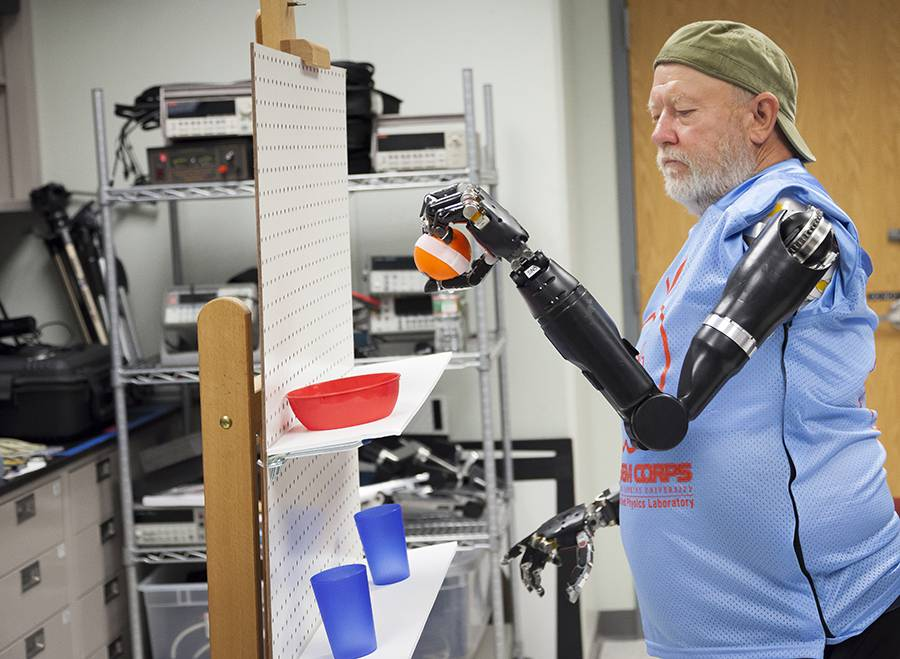
\includegraphics[width=\linewidth]{prostetic-arms.jpg}
  \caption[Les Baugh, an amputee, is using his mind to control two robotic arms to perform several tasks that require fine motor control of his arms]{Les Baugh, an amputee, is using his mind to control two robotic arms to perform several tasks that require fine motor control of his arms \citep{campbell_amputee_2014}.}
  \label{fig:prostetic-arms}
\end{figure}

It may appear evident that BCIs can significantly impact the field of therapeutics and accessibility for a small subset of the human population. However, one can envision not only alleviating deplorable living conditions but also improving the lives of healthy people through more natural or efficient ways of interacting with technology or people surrounding us or by directly altering human brains for certain benefits such as the possibility to enhance or delete bad memories \citep{spiers_enhance_2014} or record and guide dreams \citep{haar_horowitz_dormio_2020}.

Many use-cases still seem a long way from being applicable today, yet many capable people and even entire companies are developing BCI hardware and software aimed at the general population, such as Neuralink \citep{urban_neuralink_2017}. The general applicability of a BCI system to the mass market will depend on several factors, of which the form factor and invasiveness of the hardware are likely to be essential aspects. Nevertheless, the totality of the ecosystem in which the software resides is a valuable aspect that should not be overlooked.

\section{Opportunity}
\label{chapter1-opportunity}

Whether it is a bidirectional and invasive BCI or a unidirectional and non-invasive BCI, the data collected from the brain would always need to be processed, contextualised, and classified to produce an intelligible output to interface with as shown on \autoref{fig:directional-system}.

\begin{figure}[ht]
  \centering
  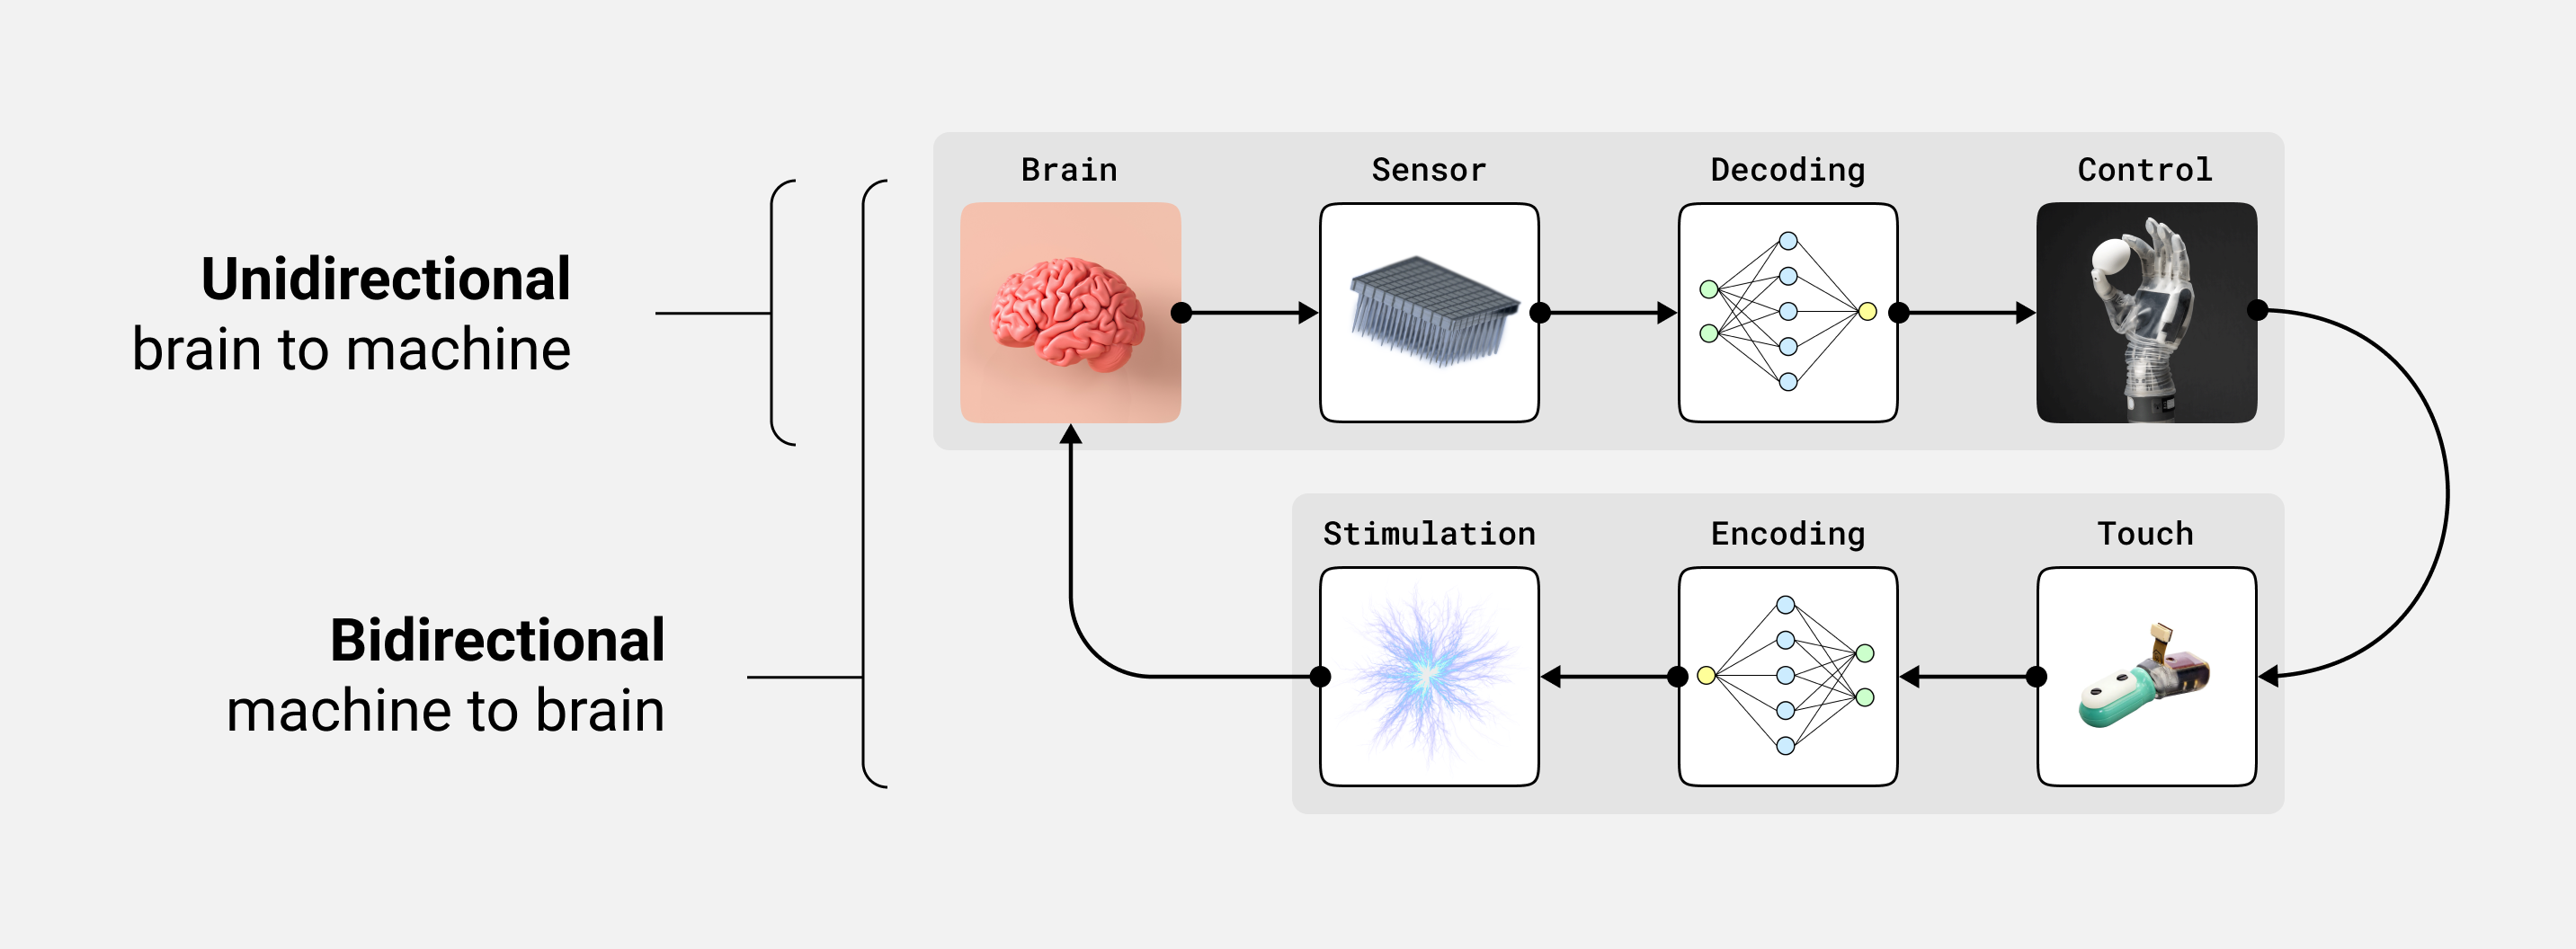
\includegraphics[width=\linewidth]{directional-system.png}
  \caption{Conceptual difference between a unidirectional and a bidirectional BCI and a simplified overview.}
  \label{fig:directional-system}
\end{figure}

Most current BCI software systems being developed, e.g. for a BCI implanted in a living patient, are typically deployed in a local environment, i.e. the software system and its components are located on a physically nearby computer.

The author sees the opportunity to move BCI software from local environments to the cloud to enable a variety of benefits for the general population and mass-market. The present thesis determines  what components such a cloud-based and mass-market-ready software system would require. The emphasis is on a holistic view of such a system, which means that the entire technology stack and context are taken into account.

\section{Supposition}
\label{chapter1-supposition}

There is already promising research on implications of brain/cloud interfaces (B/CI) by \citeauthor{martins_human_2019} \citeyearpar{martins_human_2019} or by \citeauthor{angelica_cognitive_2021} \citeyearpar{angelica_cognitive_2021}, which analyse bringing hypothetical large-scale BCI software systems into the cloud. Nonetheless, their research focuses on speculations based on hypothetical scenarios in the future, usually based on the premise of other developed technologies such as neural nanorobotics, vital advances in 5G, or the presence of supercomputers in the cloud, e.g. for the augmentation of the human brain, and are thus somewhat distant from today's pertinence. To distinguish the research presented in this thesis, the author coins the term neural/cloud interface (N/CI), which refers to a holistic software system that connects a neural interface device such as a BCI to the cloud and then to other neural interfaces, software systems, or physical devices.

The primary supposition is that a N/CI is feasible with contemporary software technologies, requiring only theoretical groundwork based on empirical software engineering. To shed more light on this, this thesis looks at the process and lessons learned from the author's perspective in developing a real-life N/CI in the industry.

\section{Goals and objectives}
\label{chapter1-goals-and-objectives}

The overall goals of this thesis are to give the reader an overview of the context and definition of a N/CI and most importantly the software components that make it up. In order to achieve these goals, the author must achieve the following objectives:

\begin{enumerate}
  \item Describe the context and motivation behind creating a N/CI.
  \item Establish a clear definition, distinction and advantages of a N/CI.
  \item Identify and define the most relevant aspects required to realise a N/CI.
  \item Illustrate an example architecture of a N/CI to implement its components in practise.
\end{enumerate}

\nomenclature[bci]{BCI}{Brain-computer interface}
\nomenclature[ecog]{ECoG}{Electrocorticography}
\nomenclature[cat]{CAT}{Computed tomography}
\nomenclature[eeg]{EEG}{Electroencephalography}
\nomenclature[bc-i]{B/CI}{Brain/cloud interface}
\nomenclature[nci]{N/CI}{Neural/cloud interface}
\nomenclature[hci]{HCI}{Human-computer interaction}
